\documentclass[10pt]{book}
%\documentclass{tufte-handout}
\usepackage{color}
\usepackage{graphicx}
%\newcommand{\beforefig}{\vspace{1.3\parskip}}
%\newcommand{\afterfig}{\vspace{-0.2\parskip}}
\newcommand{\beforefig}{\vspace{0.2in}}
\newcommand{\afterfig}{\vspace{0.2in}}
\begin{document}

\title{Abstracting, Act 2: Thermal Systems}

\section{Where we're going}

So far we've dealt mostly with modeling populations, and we have done so using discrete time models -- models where we assume, either for simplicity or for structural reasons, that it makes sense to talk about the state of the system at discrete points in time.  

To do this, we've utilized a couple of pieces of formalism: stock and flow diagrams, which qualitatively represent our understanding of what quantities we are tracking, and how they evolve in time, and difference equations, which more quantitatively express the model. 

We've also worked on implementing models, using both MATLAB and using some analytical tools (e.g., finding equilibria for a set of difference equations). We've started to validate models -- mostly using comparison to data and common sense -- and we've begun to go beyond using a model to generate a time series.

We're now going to iterate again on the modeling process.  You'll see some new stuff along the way:

\begin{itemize}
\item We will begin dealing with continuous time models -- models in which we assume that the system is evolving constantly in time, and in which we are able, in principle, to ask about what the state of the system is at any given time.
\item We'll begin looking at systems other than populations -- initially, thermal systems, and shortly after that, physiological systems.
\item We'll be seeing some new mathematical formalism -- differential equations
\item We'll be learning some new implementation approaches for differential equations -- both analytical and numerical
\item We'll be introducing some new validation ideas, such as limiting behavior
\item We'll be starting to think about how to be more sophisticated in doing work with models, both by introducing lumped parameters, and by thinking about figures of merit.
\end{itemize}

At the same time, our old friend the stock and flow is still with us, and we'll resurrect difference equations to help us make sense of differential equations -- so the territory is not really all that new...

\section{Differential Equations and Stocks and Flows: A First Encounter}

In modeling populations, we used difference equations.  For example, we modeled the elephant population in year $n+1$, $E_{n+1}$, as depending on the population in year $n$:
$$E_{n+1} = E_n + bE_n - d E_n$$
As we move into modeling thermal and other systems, we are going to begin using a different type of mathematical formalism:  the {\it differential equation}.

At its core, a differential equation is simply an equation that involves derivatives.  A very simple example would be
$$\frac{df}{dt} = 0$$
which states that the function $f$ has a derivative of zero.

While we're going to develop more sophistication with differential equations as we go along, for now it's probably easiest to think about differential equations as statements about rates of change.  For example, 
$$\frac{dx}{dt} = C(x_0-x)$$
says that the rate of change of  $x$ is proportional to how far $x$ is from $x_0$.  If $x<x_0$, then the rate of change of $x$ is positive, and if $x>x_0$, the rate of change is negative.  

Differential equations tie very directly to stocks and flows:  a flow is something that causes a stock to change, so the total rate of change of a given stock should depend on what flows are attached to it.  In general, if you are translating a stock and flow to a differential equation (or vice-versa), 
{\bf each stock should have a differential equation associated with it, and that equation should have the same number of contributions as there are flows into and out of the stock.}   

NEED A NONSPECIFIC EXAMPLE HERE.

\section{Example: Pharmacokinetic Systems}

When you take a drug -- whether it is asprin or cocaine -- a diverse set of things happen in your body.  The drug moves through your system, and is gradually broken down and/or eliminated from your system; and your body reacts in a variety of ways to the presence of the drug.  {\it Pharmacokinetics} deals with the question of how the drug moves through the body:  how long does the Tylenol remain in your stomach, your blood,  etc., while {\it pharmacodynamics} deals with the question of how your body reacts to the  drug.

While there are a variety of approaches to pharmacokinetic modeling, one attractive approach is to try to build a model that is physiologically based -- i.e., that keeps track of how much drug is where.  Such a model clealry lends itself nicely to a stock and flow picture: one can imagine keeping track of the amount of drug in the stomach, in the small intestine, in the blood, etc.  

\subsection{The most common pharmacokinetic model: First order behavior}

For a variety of reasons, many biological elimination processes can be modeled as first order behavior -- i.e., the magnitude of the flow is directly proportional to the stock.  This, if you were modeling the amount of alcohol in someone's stomach over the course of an evening at a bar, you might  draw a stock and flow that looked like this:

\beforefig
 \centerline{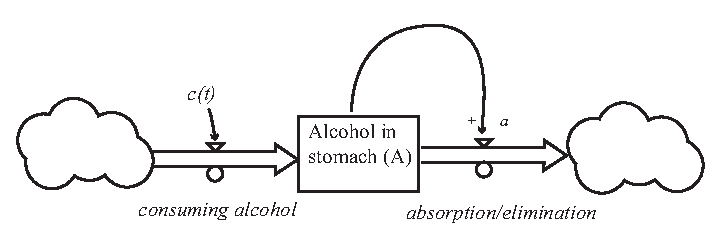
\includegraphics[height=1in]{figs/AlcoholExample1}}
\afterfig

Here the flow into the stomach, $c(t)$  is the person's alcohol consumption as a function of time, and $a$ is the elimination constant.  What would the units of $c(t)$ be?  Of $a$?

The flow out of the stomach is the elimination process.  The model's assumption the flow is controlled by the amount of alcohol in the stomach  makes quite a bit of sense physically  for low alcohol consumption levels -- if there were no alcohol, there would be none to eliminate.  At higher levels of consumption, such a model might be less appropriate:  one could imagine, for example, that the there are limits on how fast alcohol can be eliminated.

Corresponding to this stock and flow would be the following differential equation:
$$\frac{dA}{dt} = c(t) - aA$$
which states that the rate of change of the alcohol stock depends on the flow of alcohol due to consumption, $c(t)$, and the elimination rate of alcohol, which is proportional to how much alcohol is in the stomach. Note that this is pretty analogous to difference equations:  you end up with one difference equation per stock, and you also end up with one additional term in a given difference equation per flow.  

\subsection{Multiple compartments in pharmacokinetics}

Of course, a more relevant quantity than the amount of alcohol in a patient's stomach might be the patient's blood alcohol level (BAC).  A multiple stock model could be used to build a model for the time evolution of a the BAC.  For example, one possible model might look like this:

\beforefig
 \centerline{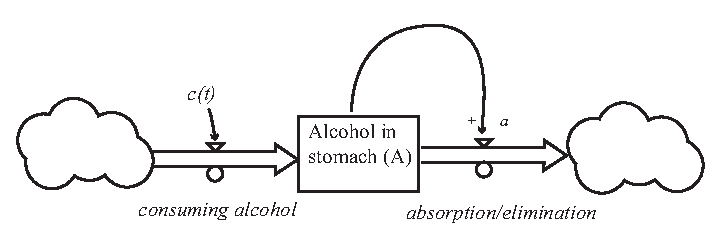
\includegraphics[height=1in]{figs/AlcoholExample1}}
\afterfig

Now the model is tracking the alcohol in the stomach and in the blood; transfer from the stomach to the blood is modeled as a first order process.  Once alcohol is in the blood, we assume that it can be removed by two processes:  it can be metabolized, or it can be eliminated by the kidneys.  For a first pass model, we'll assume both of these are also first order processes.  Thus, the differential equations for this model are
$$\frac{dA}{dt} = c(t) - aA$$
$$\frac{dB}{dt} =  aA - mB - kB$$
where $A$ is teh amount of alcohol in the stomach, $B$ is the amount of alcohol in the blood,  $c(t)$ is the rate of alcohol consumption, $a$ is the stomach to blood elimination constant, $m$ is the blood to metabolization constant, and $k$ is the blood to kidneys elimination constant.

Questions:  Why are two differential equations required?  Why does the differential equation for $A$ have two terms on the right, while the differential equation for $B$ has three?

\subsection{Disciplinary conventions and caveats}

 
 
 \section{Example: Thermal Systems}

While it is tempting to think about thermodynamics as being all about temperature, it is really a very general science that is concerned with the question of how a system changes state as a result of various processes (heat flows, work, etc.).  

That idea -- that a system changes state as a result of processes -- should sound familiar, because it's the way we've been talking about stocks and flows.  Stocks represent the state of the system (e.g., how many elephants there are), and flows represent the processes by which the system changes (e.g., hunting).  

\subsection{State Variables}

in thermodynamics, the extensive state variables that we use to describe the system -- i.e., the types of stocks -- are a bit more abstract than in modeling elephant populations.  We tend to be concerned with two different types of stocks:

\begin{itemize}
\item {\it Internal Energy} is perhaps the stock we'll encounter most frequently.  Internal energy is a measurement of the total energy contained in the system, both in the form of potential energy {\it within} the system (e.g., a compressed spring), and in the form of kinetic energy within the system (e.g., molecules moving around or vibrating).  Internal energy is denoted with a $U$, and (in SI units) has units of Joules.

\item {\it Mass} of a system can change as well, if the system has open boundaries -- i.e., if matter is allowed to go across the boundary.  Mass if typically denoted $m$, and has units of kilograms.

\item{\it Volume}, denoted $V$, can be thought of as a stock, although this requires a bit more brain stretching than mass or internal energy.  The units are, of course, meters$^3$.

\end{itemize}

While we are discussing stocks in thermal systems, it is worth highlighting that {\bf temperature is not a stock}.  This is because temperature is an intensive state variable.  Doubling the size of the system does not increase the temperature of the system, and it does not make sense to think about temperature ``flowing''.  Of course, the fact that temperature is neither a stock nor a flow doesn't mean it's not important.  Intensive state variables you are likely to encounter include:

\begin{itemize}
\item {\it Temperature}, denoted $T$, has units of Kelvins.
\item {\it Pressure}, denoted $P$, has units of Newtons/meter$^2$.
\item {\it Density}, denoted $\rho$, has units of kg/meter$^3$.
\end{itemize}

\subsection{Processes for Changing Internal Energy: Heat and Work}

The internal energy of a system can change due to heat being added to the system: put a pan on the stove, and when you turn on the flame, you will begin increasing the internal energy of the pan.   Internal energy can also be changed by doing work on the system, or by having the system do work on something else.  For example, in a car engine, expanding gas pushes up the pistons in the cylinders; this work done by the gas reduces the internal energy of the gas.  In general,
$$\Delta U = Q - W$$
where  $\Delta U$ is the change in the internal energy of the system, $Q$ is the heat that is added, and $W$ is the work done {\it by the system}.  Note that both heat and work have units of energy here.  

Heat is (rather circularly) defined as energy that is transferred by means other than doing work; examples of heat flow mechanisms include conduction (if you touch something hot, energy flows into you from the hotter object), radiation (e.g., energy flowing into your skin from the sun as you lie on the beach), and mass transfer (e.g., energy being carried away in evaporating water).  Unfortunately this definition of heat tends to be at odds with our typical usage of the word -- when we talk about ``turning up the heat'', we typically mean that we wish to increase the {\it rate} of heat transfer. Thus, we often use the word ``heat'' to refer to a flow, which, while just fine in casual usage, is very wrong indeed in the world of physics and engineering...

Work includes both traditional mechanical work (i.e., exerting a force through a distance -- as in moving a piston) and other forms of work (e.g., charging a battery).

\subsection{A Simple Example}

Let's think through a simple example to illustrate the stock and flow picture of thermodynamics.

Imagine we have a pot of water on a stove, and we're interested in knowing what will happen to it in the future.  In abstracting this, you might choose to say ``It's a mass of water, in thermal contact with one side of a pan.  On the other side of the pan is a burner.''  If you were really interested in is what happens to the {\em water}, you might say that your ``system''  is the water in the pan, and the ``surroundings'' are everything else.  Of course, you could make a different choice here -- e.g., you could decide that the system included the pan.  

\beforefig
 \centerline{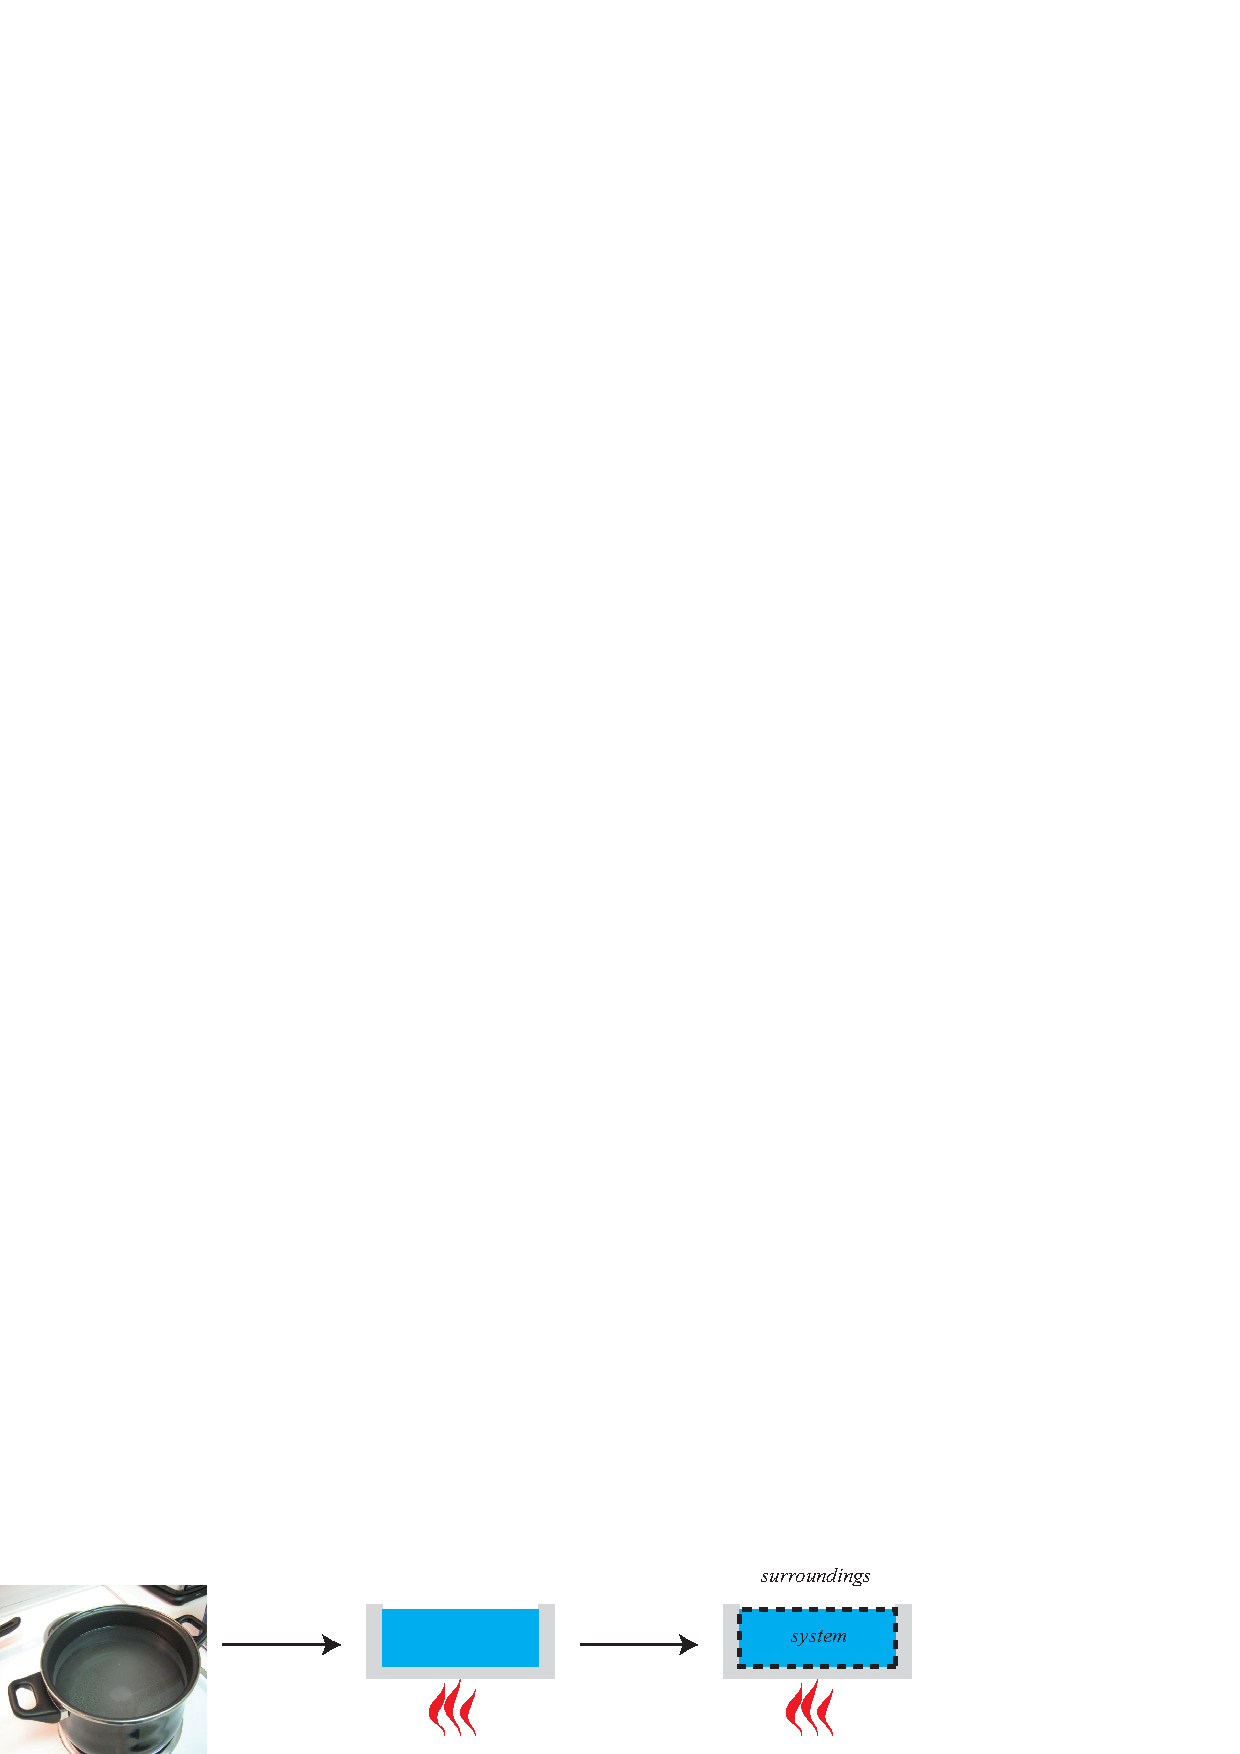
\includegraphics[height=1in]{figs/ThermalSystemAbstraction.png}}
\afterfig

Once you've decided what your system is, you need to think about what stuff can flow into and out of your system.  Clearly heat can flow in (from the burner), or out into the environment, by (for example) conduction through the walls of the pan.  And assuming that evaporation can happen (i..e, it is an open system), mass could also cross the system boundary.  Finally, note that when a water molecule crosses the system boundary, it also carries away some energy -- so it is necessary to think about energy flow due to mass flow.  Thus, two stocks are needed to keep track of the system: the internal energy of the water in the pan, and the mass of water in the pan.  And we'll need multiple flows, both to represent the loss of mass due to evaporation, and to represent the various losses and gains of internal energy we've identified.  So, a simple stock and flow (without any controls shown) might look like this:

\beforefig
 \centerline{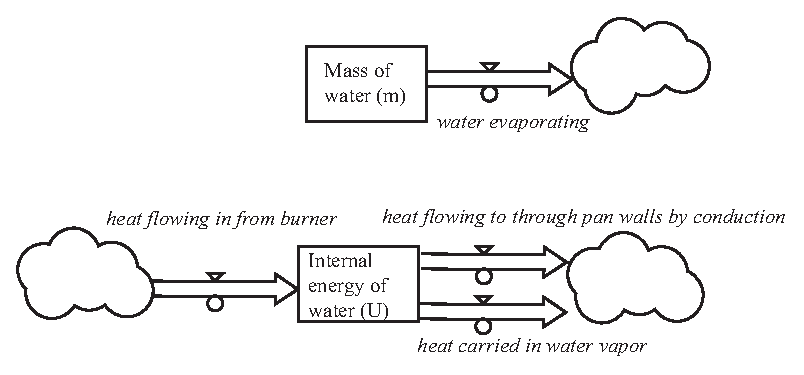
\includegraphics[height=2in]{figs/WaterInPanSimple}}
\afterfig

Of course, we've not yet defined anything about how these processes work or how to model them: the flows in this stock and flow diagram are only defined in the most hand-wavy way.  But we at least have a general picture of what is going on, and now can begin thinking about models for temperature, heat flow, etc.

\section{Thermodynamic Relationships}

In order to model the flows in a thermodynamic system, we need to deal with a couple of issues:  first, {\it how does temperature relate to internal energy?}, and second, {\it what are the mechanisms for heat flow?}.  We deal with these two questions in the following sections.


\subsection{Temperature, Heat Capacity, and Phase Change}

Although it might make perfectly good sense to talk about the amount of internal energy in a system, the reality is that this is not a quantity that we measure directly -- rather, we tend to measure temperature.  

Temperature, it turns out, is closely related to the internal energy of a system.  One way to define temperature (in statistical mechanics) is to relate it to the average kinetic energy of a particle in the system.  For example, in a monatomic gas, the average kinetic energy of an atom in the gas is given by
$$<KE> = \frac{3}{2} k_B T$$
where $k_B$ is the Boltzmann constant, a fundamental physical constant with the value of $1.380 \times 10^{-23}$ m$^2$ kg s$^{-2}$ K$^{-1}$

At a macroscopic level, this means that when you raise the temperature of a single phase system a certain amount $\Delta T$, the change in internal energy is directly proportional:
$$\Delta U \propto \Delta T$$
Things get a bit more complicated when you have a phase change.  
For example, imagine you took a kilogram of ice, put it in a container, and started to add heat at a constant rate (i.e., constant power).  What would the temperature look like as a function of time?

Below 273 K, the ice's temperature would rise approximately linearly in time.   Now, at atmospheric pressure, water changes from ice to liquid at $273$ K, and from water to steam at $373$ K.  A certain amount of energy -- the {\it latent heat} --  is required to create the phase change. So, when the temperature reached 273, it would stay there a while -- until we'd put in the latent heat of fusion required to change all of the ice into liquid.  Then the temperature would again begin to rise linearly in time, until we reached the boiling point, and so on.  Of course, above the boiling point, we'd have to start to worry more about keeping the pressure constant... but that's another story.

Thus, if we plotted the internal energy of a mass $m$ of water at atmospheric pressure as a function of its temperature, we would get a picture that looked something like this:

\beforefig
 \centerline{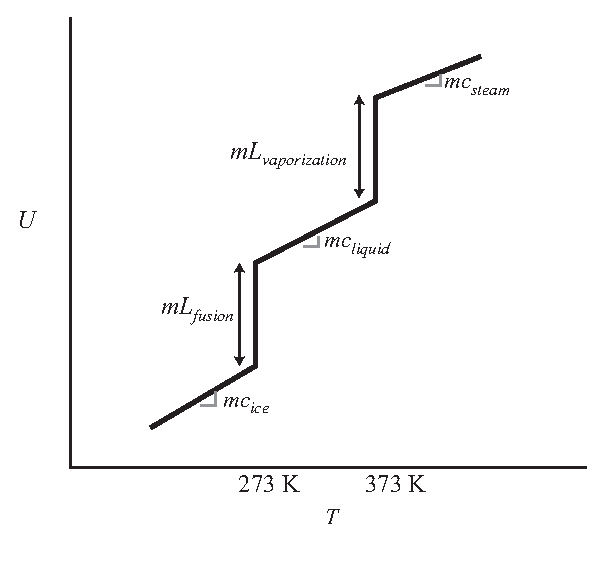
\includegraphics[height=3in]{figs/SpecificHeatWater}}
\afterfig

Note the slopes above: when the material is in a single phase (e.g., liquid), the change in the internal energy is {\it nominally} (this is a model, after all) linearly proportional to the change in temperature:
$$ \Delta U = m c \Delta T$$
where $m$  is the mass of the system, $c$ is the {\it specific heat} (units of J/K-kg), and $\Delta T$ is the change in temperature.

In order to change phase, the internal energy must rise an additional amount,
$$\Delta U = m L$$
where $L$ is the {\it specific latent heat} of the system (units of J/kg).

Often we'll talk about the {\it heat capacity}, or {\it thermal mass} of a system, $C = m c$.  This simply tells you what the change in internal energy is per change in temperature, i.e., the amount of energy required to raise the temperature 1 degree:
$$C = \frac{\Delta U}{\Delta T}$$ 
Note that $c$ and $L$ are intensive properties, whereas $C$ is extensive.

\subsection{Mechanisms for Heat Transfer}

\subsubsection{Just tell me the power}

In some situations, heat transfer can be thought of simply as a constant power process.  For example, if you put a 500 W immersion heater into a cup of water, it's a pretty good model to simply assume that the 500 W heater is delivering 500 W to the water.  Thus the rate of change of the internal energy would be
$$\frac{dU}{dt} = 500 W$$
Your metabolism acts a bit like an immersion heater -- the basal metabolism rate is around 60 W.

When you are lying in the sun, you are absorbing solar radiation at a pretty constant rate: insolation (incident solar radiation) has a particular value for a given location, weather condition, and time of day -- for example, at noon at sea level, insolation is about 1000 W/m$^2$.  Your body, of course, reflects some of the radiation, so that your rate of change in internal energy will be given by 
$$\frac{dU}{dt} = e I A$$
where  I is insolation in W/m$^2$, A your effective surface area in m$^2$ and e is the efficiency of absorption.  Note in this example that you have to be a bit careful when you define $A$:  it is the projected exposed surface area:


\beforefig
 \centerline{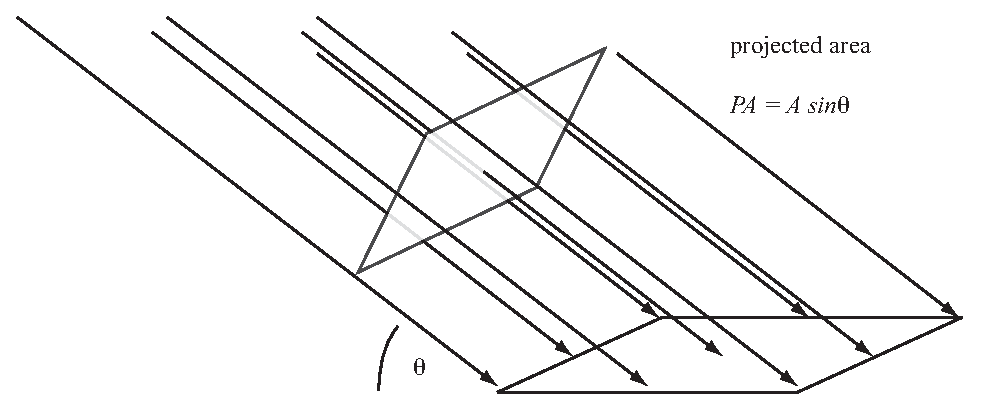
\includegraphics[height=1.5in]{figs/ProjectedArea}}
\afterfig

\subsubsection{Conduction: Heat Transfer by Vibration}

{\it Conduction} is a heat transfer mechanism that involves heat flow through matter, due to differences in temperature between one point and another.  In conduction, the physical mechanism for heat transfer is vibration of particles, as opposed to bulk motion of particles. For example, if you hold a metal rod, and stick one end into a campfire, the atoms in the rod at that end absorb energy from the fire, and start to vibrate more.  These vibrating atoms knock into their neighbors, causing them to vibrate, and so forth.  Thus, the end that you are holding will eventually get hot as energy is carried down the rod by these vibrations: heat flows from the hot end to the cold end, which leads to the cold end getting warmer. 

Conduction is typically modeled using Fourier's law (which is, of course, a very good model, not a law).  Basically Fourier's law is a version of effort and flow (yay, ModCon!):  the power (heat flow) is proportional to the temperature difference.  If we consider two bodies in thermal contact,  the rate of change of the internal energy in each body is given by
$$\frac{dU_1}{dt} =  -K(T_1 - T_2)$$ 
$$\frac{dU_2}{dt} = K(T_1 - T_2)$$ 
where $T_1$ and $T_2$ are the temperatures of the bodies respectively, and $K$ is the total {\it thermal conductance} between the two bodies, which measures how easily heat travels from one body to the other.  Note that the units of $K$ here are J/K.

Let's think about an example of this:  a styrofoam cooler, containing a block of ice at 260 K, is placed in a room that is at 300 K.  How would we describe conduction through the walls of the cooler?

We'll start by thinking about how to abstract this.  We'll define our system as the ice, and the only stock we care about is the internal energy of the ice (since no mass will enter or leave the system -- i.e., I'm assuming sublimation is not important.  The flow of energy into the cooler from the environment will be governed by a few things:  the environmental temperature, the temperature of the ice (which, in turn, depends on the internal energy of the ice), and the conductance of the cooler's walls.  So, qualitatively, we might represent the model like this:


\beforefig
 \centerline{\includegraphics[height=2in]{figs/IceInACoolerAbstraction}}
\afterfig

Now, if we want to get quantitative about this, we'll need to somehow figure out (1) how to get the temperature from the internal energy (which involves re-reading the section above!), and (2) how to determine the thermal conductance of the cooler.  Referring back above, I'll claim that
$$T_{ice}=260 + \frac{\Delta U_{ice}}{c_{ice}m}$$
where $\Delta U_{ice}$ is the change in the internal energy of the ice from the point at which $T=260$ K.

Thanks to the wonders of the world wide web, I find that styrofoam has a thermal conductivity of 0.033.  When I look a little closer, I find the {\it units} of this thermal conductivity to be W/m-K.  

Now, this thermal conductivity that I've just looked up is denoted $k$ (as opposed to $K$) -- it is an intensive property of the material, NOT the total thermal conductance of the walls of the cooler.  I need to somehow translate this intensive property into a quantity specific to the system.  Well, a wall with a larger surface area will conduct more (i.e., bigger houses lose more heat through the walls than smaller houses).  So, I expect the total thermal conductance to be proportional to the surface area through which the heat is traveling.   Furthermore, the thicker the wall, the less heat I expect to travel through.  Thus,
$$K = k A/d$$
where $A$ is the surface area (here, the area of the cooler), and $d$ is the thickness of the walls.  Assuming my cooler is $0.2 \times 0.2 \times 0.3$ meters with a wall thickness of 4 cm,  the total surface area is $2\times 0.04 + 4 \times 0.06$ m$^2$, yielding $K = 0.033 \times 0.32 /0.04 = 0.264$ W/K.
So, the rate of change of the internal energy will be given by
$$\frac{d\Delta U_{ice}}{dt} = K (T_{env}-T_{ice}) = 0.264\left(300 - \left(260+\frac{\Delta U_{ice}}{c_{ice}m} \right) \right)$$
Note that our final differential equation here does not explicitly contain the temperature of the ice; rather it expresses the rate of change of internal energy in terms of the internal energy.

One of the confusing things about this model is the extent to which a body with a heat capacity can, in itself, be a thermal conductor.  For example, when you foolishly put one end of a metal rod in a campfire, the rod's internal energy increases, and at the same time there is heat flow within the rod.   Similarly, in a house, the walls of the house both conduct heat to the outdoors, and hold some amount of the house's internal energy.

One way to deal with this is to separate the object into one or more lumped thermal masses, connected by appropriate thermal conductance(s).  For example, we might choose to break the rod into two parts, or three parts, or four parts, or 1000 parts:

\beforefig
 \centerline{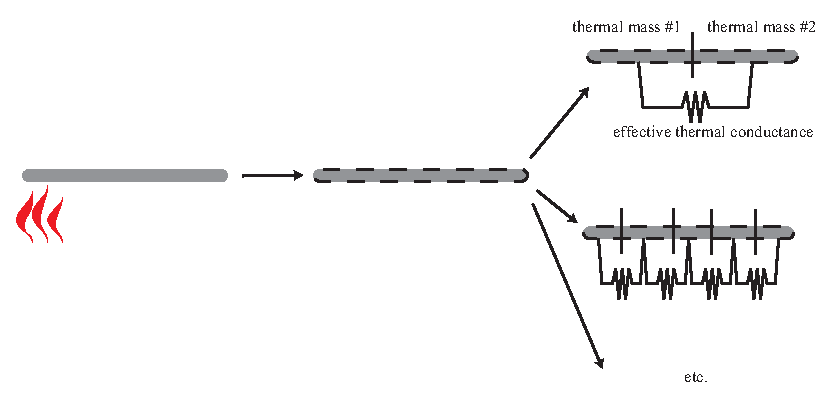
\includegraphics[height=2in]{figs/BreakingUpARod}}
\afterfig

Later (like next semester) we'll deal with this in more detail -- for now, the key idea is that you pull the stock apart from the flow:


\beforefig
 \centerline{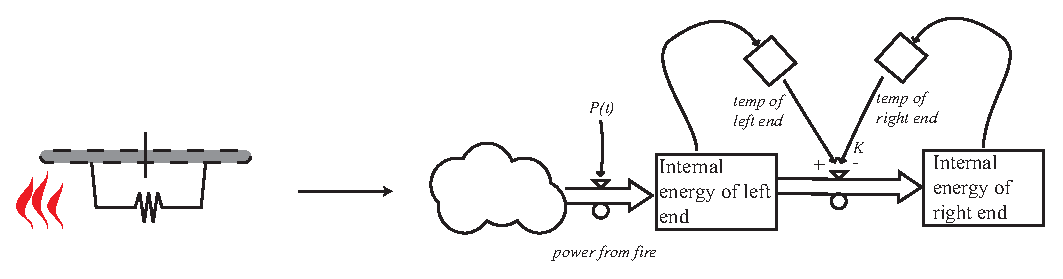
\includegraphics[height=1in]{figs/RodStockAndFlow}}
\afterfig

When you decide how to break things up, it's important to think about the {\it relative} conductance of different parts of the system.  For example, if half of your rod was made of gold (which has a very high thermal conductivity) and the other half was made of wood (with a low conductivity), you would likely NOT want to break the gold portion up -- heat will travel much faster in the gold than in the wood, so it's probably safe to guess that the temperature of the gold will be relatively uniform -- so breaking the gold up into little chunks might not be worth the effort. 

\subsubsection{R Values, U Values, K Values, and all that}
It is worth taking a moment to highlight some of the different ways that thermal conductivity, conductance, resistivity, and resistance are talked about.

Thermal {\it conductivity} is an intensive material property -- e.g., styrofoam, regardless of its shape, has a particular thermal conductivity -- and it tells you how well a particular type of material conducts heat.  Higher thermal conductivity implies that heat travels more easily in the material.  Thermal conductivity is denoted with a lower case $k$, and (in SI units) has units of W/K-m.  Typical values of $k$ range from about 0.04 W/K-m for fiberglass insulation to 400 W/K-m for copper.
Thermal {\it resistivity} is simply the inverse of thermal conductivity; usually you'll find conductivity listed, though.

Thermal {\it conductance} is a property of a given configuration of a particular material that connects one thermal mass to another.  It describes the rate of heat flow between the two bodies for a given temperature difference.  As argued above, for a wall of area $A$ and thickness $d$ with thermal conductivity $k$, the thermal conductance through the wall is given by $K = \frac{kA}{d}$, and the heat flow (power) from body 1 to body 2 is given by $K(T_1-T_2)$.  The units of thermal conductance are W/K.

Thermal {\it resistance} is simply the inverse of thermal conductance.  

Now, if that weren't confusing enough, you will also find things called $R$ values and $U$ values when you look around for windows or house insulation.  For example, you might buy some "R19" fiberglass insulation.  What does this mean, exactly?  Well, $U$ values are conductance per unit area:  the total conductance of a wall of area $A$ and $U$ value 0.1 is $K = 0.1 A$.  If you think through the units here, you'll see that $U$ value has units of W/K-m$^2$ in SI.  Of course, in the U.S., most $U$ and $R$ values are given in archaic British units:  the units of $U$ are BTU/hr$^{\circ}$F ft$^2$ (sigh...).  $R$ value is simply the inverse of $U$ value.

Adding thermal resistances and conductances is just like adding electrical resistances and conductances:  resistance adds in series (e.g., if you have two layers, like a wall with R19 insulation, followed by a second wall with R19 insulation, the effective R value of the double-thick wall is R38); conductance adds in parallel (e.g., for a house, $K_{total} = K_{roof} + K_{walls} + K_{floor}$).

{\bf Exercise:}  A cubic block of copper, at room temperature, is encased in R30 insulation.  The insulated block is then placed outside on a cold day.  You are asked to predict how the temperature of the block will change.
\begin{enumerate}
\item Create a control volume picture for this situation.
\item Find a differential equation for the internal energy of the block.
\item Find a differential equation that tells you the rate of change of the temperature of the block in terms of the outside temperature, the block's temperature, and the block's mass. 
\item Use your differential equation to calculate the rate of temperature change of the block for $T_{block} = 30 ^{\circ}$C, $T_{outside}=0  ^{\circ}$C, and $m_{block}$=10 kg. 
\end{enumerate}

 
\subsection{Radiation: Heat Transfer by Light}

{\it Radiation}, as a heat transfer mechanism, is the transport of heat by emitted photons (i.e., light) due to the thermal motion of charged particles in a body.  In contrast with conduction, where the energy is carried by vibrations, in radiation, the energy is carried by light.  For example, when you turn on a space heater or an electric stove, the electrons and protons in the heating element begin to shake around more as the temperature of the element rises, and consequently the heating element begins to glow (emit visible light).

Much of the light that is emitted due to thermal radiation is infra red -- too long a wavelength to see -- but you can still very much feel thermal radiation (e.g., even before the heating element begins to glow, you can still hold you hand above it and feel the radiated heat).

So long as an object's temperature is above absolute zero (i.e., any object in the universe), it will  radiate some amount of power.  The power emitted (and hence the rate of loss of internal energy) is strongly dependent on the temperature of the object, and also depends on the object itself:
$$P_{emitted} = -\frac{dU}{dt}  = e \sigma A T^4$$
where $A$ is area of the object (which we have to think carefully about), $T$ is temperature of the object (in Kelvin), $e$ is the emissivity of the surface of the object, and  $\sigma$ is the Stefan-Boltzmann constant., which has a value of $5.67\times 10^{?8}$ W/m$^{2}$K$^4$.  Emissivity is a material property, which ranges between near 0 for shiny stuff (e.g., for aluminum foil, $e=0.04$) and near 1 for dark, dull stuff.  Human skin has an emissivity near 1.

Now if you think about it, this sounds a bit weird -- everything is giving off energy all the time??  Wouldn't we all be getting colder as a result?  The tradeoff, of course, is that things are constantly absorbing radiation from the environment as well.
  In fact, it turns out (and can be fairly easily proven) that the absorbtivity of a surface is equal to its emissivity:  if you shine a flashlight with power $P$ on a surface, the time rate of change of the body's internal energy will be given by
$$\frac{dU}{dt}  = eP$$
and when a body is in an environment of temperature $T_0$, it is absorbing energy at a rate of 
$$P_{absorbed} = +\frac{dU}{dt}  = e \sigma A T_0^4$$
Because of the $T^4$ dependence, radiation becomes very important in cases where there are high temperatures involved.  It also is very important in cases where other mechanisms (e.g., conduction, convection) are not present.  For example, in vacuum, convection and conduction are zero, since there is no matter to carry the heat, so radiation is the only relevant mechanism. 

\subsubsection{Exercise: Freezing in Space}

In the cold, dark depths of space, the temperature is near to absolute zero.  Furthermore, the level of solar radiation can be quite high (e.g., at the distance of the earth from the sun, the solar insolation is 1366 $W/m^2$.  

Consequently,  at least according to wikipedia, one important requirement for space suits is  temperature regulation:

``Unlike on Earth, where heat can be transferred by convection to the atmosphere, in space heat can be lost only by thermal radiation or by conduction to objects in physical contact with the space suit. Since the temperature on the outside of the suit varies greatly between sunlight and shadow, the suit is heavily insulated, and the temperature inside the suit is regulated by a Liquid Cooling Garment in contact with the astronaut's skin, as well as air temperature maintained by the Primary Life Support System.''

Do you buy this?  How bad would it actually be if your space suit consisted of (say) a thin layer of shiny foil?  Would you freeze?  Would you burn up?  (set aside the pressure regulation question for now, although you might be interested in looking up Space Activity Suits to learn more about this...). 

\subsection{Convection: Heat Transfer by Mass Transfer}

The third way to transfer heat is by the actual motion of particles - think back to the water vapor leaving the pan, and carrying away energy in doing so.  A very simple example occurs when you open the door of your house on a cold day: warm air exits your house (carrying energy out) and is replaced by cold air from outside (which has less internal energy than the warm air it replaced).  Thus, opening the door of your house results in a net drop in your house's internal energy.  A more complex example is convection currents: temperature differences within a fluid can result in currents that not only move material around in the fluid, but also transport heat from one location to another. Most of the earth's weather is driven by convection processes.

Although it is easy to understand how convection leads to heat transport, there is not one uniform model for convective processes, as they often involve complex fluid dynamics.  Having said that, there are many situations in which you can build useful models for convective heat loss without getting into the weeds of fluid dynamics.

\subsubsection{Volumetric Transfer}

Consider the case of going through a revolving door on a cold day.  When you do this, you exchange a volume $V$ of warm interior air for the same volume of cold, nasty exterior air.  Thus, this will lead to a change in internal energy of
$$ \Delta U = - V\rho c (T_{in} - T_{out})$$
where V is the exchanged volume of air, $\rho$ is the density of the air, and $c$ is the specific heat of the air.

Similarly, most houses lose air continually through poorly sealed windows, vents, etc.  If we assume that the rate of exchange is $\frac{dV}{dt}$ m$^3$/sec, the rate of change in the internal energy would be 
$$\frac{d\Delta U}{dt} = - \frac{dV}{dt} \rho c (T_{in} - T_{out})$$
This works as long as the flow is slow enough that the exiting air is at internal temperature.

\subsubsection{Boundary Layers}

Even when the actual mechanism of heat transfer is convection, it is often convenient, and accurate enough, to use a conductive model, by introducing an abstraction called a {\it boundary layer}. The basic idea here is that we imagine there is some thin layer of fluid near the interface that can be treated as if it were a thermal resistance.  

This is, in fact, not a crazy idea -- when an object is in a moving fluid, the velocity of the fluid at the surface of the object must be zero, and there is a thin distance (the boundary layer) over which the velocity rises to reach the free stream velocity.  This thin layer does tend to dominate the heat flow -- once heat gets to the free stream, it is quickly carried away.  Of course, convection {\it is} taking place within the boundary layer -- we are simply saying that the behavior of the boundary layer {\it looks like} conduction.  

Qualitatively, this model has explanatory power.  Think, for example, about a person going outside on a cold day.  The flow of heat out of the person will depend on the total thermal resistance that separates the person's core from the environment.  This total resistance will include:
\begin{itemize}
\item The thermal resistance of skin, fat, etc.: We abstract the person into a core (stock of internal energy) and a thermal resistance that connects that core to the surface of the body
\item The thermal resistance of air trapped between clothes and skin
\item The thermal resistance of cloth
\item The effective thermal resistance of the boundary layer
\end{itemize}
Qualitatively, this model says:
\begin{itemize}
\item Skinny people will get cold faster, because they have relatively low resistance between the core and the surface of the body
\item Goosedown coats will work well, because they increase the thickness of the trapped air layer
\item Heavy coats will work well, because they increase the resistance of the cloth
\item People will tend to get colder faster when it is windy, because the thickness of the boundary layer decreases with increasing wind speed.
\end{itemize}
Making this model quantitative requires some additional information / experimental results.  One option is to approximate the boundary layer thickness using a fluid dynamics approach (see wikipedia); another option would determine the thickness by comparing the time for heat to diffuse with the time for the fluid to travel over the object (see Sanjoy's book).  Either of these approaches will give you reasonable qualitative results; doing better will really require you to validate your heat transfer coefficient with some kind of empirical data.

\section{Case Study: Modeling a Solar House}

While it would be possible to do thermal modeling on elephants, it might be more interesting to think about a real situation -- for example, {\it how ought one to design a passive solar house?} 

\subsection{What was Frank thinking?}

In 1944 Frank Lloyd Wright designed the Jacobs II house.  This house,
located in Middleton Wisconsin, included multiple design features
intended to take advantage of passive solar heating: the house faces
south with a wall of glass; the house is only one room deep, so that
all rooms can benefit from solar heating, and the roof overhang is
designed to keep out summer sun while admitting winter sun.

%\begin{marginfigure}
%\includegraphics[width=6cm]{JacobsHouse.jpg}
%\caption{The Jacobs II House.  The glass facade faces south to
%  maximize passive solar heating.  Image from {\tt www.dgunning.org}.}
%\end{marginfigure}

Despite these design features, recent owners of the house have
required thousands of gallons of oil each winter to keep the house
warm\cite{BuildingBalance}. Temperature dynamics in the Jacob's house
are largely to blame for the enormous heating cost of this seemingly
well-designed house.  The original owners of the house reported that
the house's heating system would often turn off by 9AM on sunny winter
days---but they also reported that the house was so cold in the early
morning that they would have to all dress together in the bathroom, as
that was the warmest room in the house.  While
the house is well-designed for solar heating, it is not well-designed
for heat retention---it is almost completely uninsulated, and
(perhaps) lacks sufficient thermal mass.

\subsection{What kind of work do we want to do?}

We have now identified a physical situation -- the Jacobs II House.  Could we do any work with a model of this house?  What kinds of models would be required for the different types of work?

Clearly one type of work might be explanatory:  we could build a model that could help us to understand {\it why} the Jacobs II house performs as poorly as it does.  such a model might allow us to conclude that the real problem is lack of thermal mass as opposed to poor insulation.

We could also build a model that would allow us to do predictive work: the model might help us to predict what the house would be like during the summer, or to predict what would happen if we were to increase the thermal mass or increase the insulation.

FInally, we could build a model that would help us do design work.  Such a model might tell us which strategy for improving the house performance was most desirable, and potentially could tell us exactly how much to change different aspects of the design.

While the model required for all three types of work would be similar, the level of fidelity required for design work is, of course, much higher than that required for explanatory work:  for an explanatory model, it's probably OK if we get about the right values for the insulation, thermal mass, etc., whereas for design work, one would likely want a model that was more accurate with respect to parameter values, and that was also more accurate with respect to including different effects.  For example, if you are designing a house, you might like to know about local weather patterns -- something that would clearly not matter much for an explanatory model.

\subsection{Creating a Game Plan}

Let's take a minute to think about our overall game plan.

First, we should probably spend some time building a really simple model -- a very simple prototype --  even before we know much about the Jacobs II house.  While all houses are different, we probably know enough about the house right now to build a model that at least captures the right qualitative behavior. 

Why would we want to build the model before we investigate the details of the house?  Well, the model will likely give us some insight into which details are worth investigating.  If you haven't spent some time thinking about what data you need, you can end up spending a great deal of time getting swamped with details.  Furthermore, by building a model without a lot of detail, you force yourself to make a lot of simplifying assumptions.  You can, of course, refine these assumptions later -- it's always easier to go from a simple model to a more complex one, rather than vice-versa.

With a simple model in hand, we'll learn what we can from this first prototype, and in particular we'll ask two questions: {\it what kind of work this first model can do for us, and what changes would make it more powerful?}  Likely a first pass model will give us an overall impression of the behavior of the system, but will not do much more than that -- and so it's probable that we'll decide that the first prototype model is insufficient, and that we need to create improved  prototype models.   

We'll then try to identify and prioritize ways to improve on this model: should we incorporate precise geometry?  Accurate seasonal modeling?  Heat transfer between rooms in the house?  The effect of opening and closing the doors?  Deciding which of these improvements to undertake will certainly involve some research, and probably additional simple models. Additional iterations of the model will almost certainly  involve changing parameters, and could well involve structural changes from the first model.  And with each iteration, we'll again ask what we can learn from this particular iteration -- and whether an additional iteration is worthwhile.

\subsubsection{A Very, Very Simple Model}

As noted above, our first step is to make as simple a model as possible. What assumptions can we make to keep things simple?  Since this is a real-world problem, it's very tempting to start looking up all kinds of data:  the weather patterns in Madison Wisconsin, exactly what the dimensions and geometry of the house are, the exact materials the house is made of, etc.   We should resist this temptation:  those details can be added later, {\it after} we've built a very simple, but WORKING model for the house.  Too often in modeling it's possible to let the trees obscure your view of the forest; working at a high level of abstraction can help you avoid getting stuck in the weeds and mired in mixed metaphors.

So, with that warning in mind, what does the simplest possible house model look like?  My first model is going to be an order-of-magnitude model: one that gives me a sense of what the approximate numbers might be for this situation, and that helps me to think about whether my overall picture of the house makes any sense at all.   Such an order-of-magnitude model will also help me decide what {\it not} to include in the model.

For this estimation model, I'd like to treat the house as a single stock of energy.  Power flows into the house from the sun; power flows out of the house due to the temperature difference between the inside and the outside.  If the house is working well, I expect that the total amount of energy that flows out of the house over a given 24 hour period is the same as the total energy that flows in -- i.e., the average internal temperature of the house should be constant over the course of a week or a month. 

So what should we think about with respect to power flowing in and power flowing out?

Let's first think about power flowing out.  Loss mechanisms include:

\begin{itemize}
\item radiation
\item conduction through the walls and windows (including conduction through the boundary layer of air surrounding the house), and
\item volumetric losses.  
\end{itemize}

It's possible that all three of these effects are important.  What does your intuition have to say about this?  

My intutition tells me that conductive loss is probably the most important mechanism -- the house is poorly insulated; radiation tends to be more important at high temperatures which are not present in the system; and according to the owners, the heat loss occurs over night -- when the doors are presumably closed.  

But let's run some quick numbers to check our intuitition.  To estimate these we need some sense of the house's properties.  Let's estimate them.  VERY nominally, the house is something like 20 meters x 5 meters x 6 meters, so it has a volume of around 600 m$^3$, and a surface area of about 500 m$^2$.  These numbers are clearly not right, but they are not off by more than a factor of 2.
 
We'll start by looking at conductive heat loss.  The large windows will likely dominate, as the conductivity of glass is higher than that of wood and air (1 versus 0.1 W/m-K), and the thickness of the glass is much lower than the wall thickness.  For the sake of argument, assume the glass is 1 cm thick (a VERY thick pane of glass), and that the glass surface area is 100 $m^2$ (probably a bit high, so this will offset my overestimate on thickness).  This would yield a conductance of 
$$ K_{glass} = k A/d = (1) (100)/.01 = 10^4 W/K$$
In comparison, if we check out what the wall conductance might be, we could assume a total wall thickness of (say) 3 cm (including both interior and exterior walls) yielding
$$ K_{wall} = k A/d = (.1) (500)/.03 = 1.6\times 10^3 W/K$$
So we conclude the glass will be critical, even if we ignore the effect of airspace between the inner and outer walls.
We also should think about the ``boundary layer'':  what is the effect of the air on the outside (and inside) of the glass?  Well, typical heat transfer coefficients for air are between 10 and 100 W/m$^2$-K.  So the conductance of the air will be fairly high:
$$K_{air} = hA = 10^4 - 10^5 W/K$$
for the air on the surface of the glass.  This conductance is similar to the conductance of the glass itself, so we probably should think about the air and glass in series, which gives us an effective conductance for the glass of about
$$K_{effective} = (\frac{1}{K_{air}}+\frac{1}{K_{air}}+\frac{1}{K_{air}})^{-1} \approx 3 \times 10^3 W/K.$$
Note that this also implies that about 2/3 of the temperature drop will take place inside and across the glass.

If we take this conclusion and assume that the inside of the house is at 30 degrees C (an awfully high internal temperature!), and the outside is at 0, we can estimate the total power loss due to conduction:
$$P_{conduction} = K(T_{in}-T_{out}) \approx (3 \times 10^3)(30) = 9 \times 10^4 W$$ 

Now, does that make sense?  90 kilowatts? It sounds pretty big -- and we haven't dealt with other heat loss mechanisms: radiation, and also volumetric heat loss! Let's analyze these other mechanisms, and then return to the question of whether this is sensible. We'll start with radiation.

We just figured out that a good deal of the temperature drop occurs inside the house and across the glass.  So we'd expect, in the case above, that the outside of the house might be 10 degrees warmer than the environment -- at worst.  Continuing with a worst case analysis, we also will assume that the house is entirely black (i.e., emissivity of one -- not an unreasonable assumption, actually).  Given these assumptions, the total radiative power from the house is
$$P_{emitted} -P_{absorbed}= e \sigma A (T^4-T_0^4) = (1) (5.67\times 10^{-8})(500)[283^4-273^4) \approx 2.4 \times 10^4W$$

Hmm...  That's a fair bit of radiative heat loss, but then we did assume that the entire exterior of the house was at 10 degrees -- which is a pretty significant over-estimate.  Even with this assumption, we still are dominated by conductive loss through the windows.

FInally, let's think about the volumetric loss.  It's a bit hard to say exactly how much air is exchanged when you open the door of your house, but given that revolving doors are considered efficient, it's a good bet that the volume would be at least somewhat larger than the volume exchanged by a revolving door.  based on this observation, I'll estimate that we exchange 5 m$^3$ of air each time we open and close the door (that's pretty generous -- but that's OK, because I want to get a worst case sense of things!).  Over the course of a day, a family of five might go in and out of the house 20 times perhaps,  yielding a total volume of 100 m$^3$ per day.  Thus, the total energy loss per day is
$$ \Delta U = - V\rho c (T_{in} - T_{out}) = (100 m^3) (10^4 J/kg-K)(1.2 kg/m^3)(30 k) \approx 3.6 \times 10^7 J$$
So the average power loss over the course of the day is about 400 Watts -- nothing compared to the conductive heat loss!

So, in summary, our first pass at figuring out {\it losses} gives us a total loss on the order of $10^5 W$, and that loss appears to be dominated by loss through the windows.  $10^5$ Watts is not insignificant!  But does it make sense?  Well, the home owners reported using ``thousands of gallons'' of oil each winter.  A gallon of oil contains $1.4\times 10^8$ Joules of energy.  So if the house were using $10^5$ W, the oil usage would be on the order of 2.5 gallons an hour, or about 5000 gallons of oil over the course of three months.  Now there are all kinds of issues we've not considered in coming to this conclusion (the efficiency of the furnace, the gain due to passive solar, etc.) but at least it appears that our estimates might be credible, based on the data we have available.

Now that we've thought about losses, let's also make a quick first-pass model for solar gains.  As noted above, at the earth's surface, solar insolation can yield up to 1000 W/m$^2$.  Assuming that we have 100 m$^2$ of glass, the best we could possibly hope for would be a power input from the sun of $10^5$ Watts.  This sounds OK, given that the average loss is $10^5$, until you start to  consider the fact that during the winter, the sun is up for perhaps 8-10 hours per day, and the average {\it effective} area for solar insolation is likely much lower -- perhaps by a factor of 2 or 3.  In sum, it looks as though the average solar power over the course of a 24 hour period is perhaps $2 \times 10^4$ Watts. Thus, although the instantaneous power from passive solar could be similar to, or even greater than, the loss, on average the house is losing an enormous amount of energy.

Finally, let's spend a moment thinking about thermal mass.  Based on the reports, we can guess that the thermal mass must be small enough that the house can become uncomfortable in a relatively short amount of time -- maybe two hours.  Let's we assume that in the morning we're getting maximum power input from the sum (the sun is low, so the projected area of the windows will be relatively large, and that the heating system is doing enough to offset the losses due to conduction.  An uncomfortable temperature might be ten degrees above the ``normal'' temperature (e.g., 35 degrees C versus 25 degrees C).  Thus, the thermal mass of the house must be low enough that a couple of hours -- say $10^4$ seconds --  of maximum solar gain is sufficient to raise the temperature ten degrees or so.  The change in internal energy is related to the temperature change by the thermal mass:
$$ \Delta U = P \Delta t = C\Delta T$$
where $P$ is the power input (about $10^5$ Watts), and $C$ is the heat capacity, or thermal mass, of the house.  Thus, we conclude that for the house,

$$C \approx \frac{(10^5 W)(10^4 sec)}{10^{\circ} C} = 10^8 J/^\circ C$$ 

  

we can guess that the thermal mass

So our back of the envelope model allows us to reach several conclusions:
\begin{itemize}
\item First, the model seems to be consistent with the observed behavior in the house -- so we have some reason to guess that our assumptions about mechanisms, relative dimensions, etc., are not too far off.
\item Conduction, particularly through the windows, is the most important heat loss mechanism for the house, by a good margin.
\item 

\end{itemize}




Let's think about this for a winter day.  If we assume that the average inside temperature of the house is a comfortable 25 degrees C, and that the average outside temperature is  a chilly 0 degrees C.  This means that the average power leaving the house due to conduction is 
$$P_{conduction} = K (T_{in} - T_{out})$$



Well, one assumption we'd probably want to make is that the energy stored in the house can be treated as a single stock -- i.e., we are not going to concern ourselves with the details of how energy moves around inside; rather, we'll focus only on how energy moves into/out of the house.  Given that we are interested in understanding the passive solar performance of the house, it might also be reasonable to build a model that does not include a furnace (we can always add one later if we think it's important).   So, we'll assume that there is a stock of thermal energy stored in the house (probably mostly in that stone wall on the north side!). That internal energy changes due to a few processes:  sunlight coming into the house, and heat being lost by conduction through the roof, walls, windows, and floors. So, without doing ANY calculations, or looking anything up, we can sketch a stock and flow for the system:

\beforefig
 \centerline{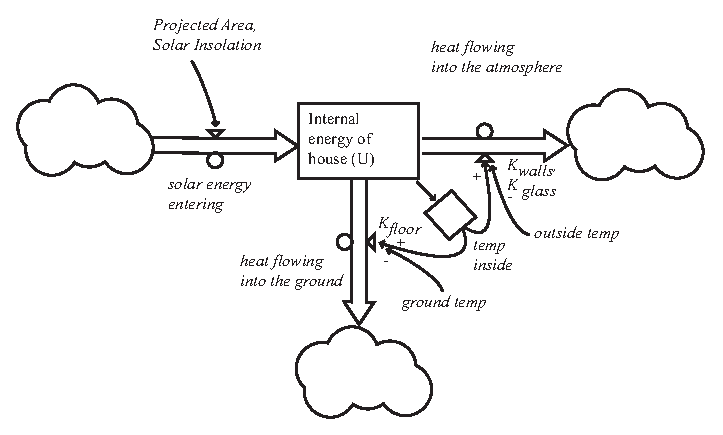
\includegraphics[height=2in]{figs/JacobsModel}}
\afterfig

Of course, once we have a stock and flow, it's also easy to write down a differential equation that describes the rate of change of the internal energy of the house:
$$\frac{dU}{dt} = eIA - (K_{window}+K_{walls}+K_{roof})(T_{in}-T_{out}) - K_{floor}(T_{in}-T_{ground})$$
where $U$ is the internal energy of the house, $eIA$ is the total solar insolation, the $K$'s are the conductances of the various parts of the house, and $T_{in}$, $T_{out}$, and $T_{ground}$ are the (changing) temperatures of the interior, exterior, and ground.




Well, first let's be clear about what we are going to model.  I propose that we should ultimately be interested in a model that tells us the temperature in the house as a function of time over the course of a typical (or perhaps not so typical) winter day.  I'll assume that we are only interested in the winter time:  the house is designed so that the summer sun is blocked,  and it appears that the house's performance difficulties are limited to the winter.  So why model the summer?


Now you might think that we're done at this point -- after all, we have a 


 (which will, of course, depend on the time of day, the geometry of the house

Second, we need to decide what effects we think will matter.  One consideration will be the energy inputs to the house.  Solar radiation clearly  is going to be important here:  it is, after all, a solar house.  The amount of solar power that gets into the house at any given time appears to depend on the geometry of the house, which is sufficiently interesting that it at least bears some consideration.   And, while it is true that the homeowners do end up using the furnace a lot, I propose that we ignore the effect of the furnace -- after all, we'll 

\subsection{Rules of thumb, and the need for a model}

In order to avoid problems like those seen in the Jacobs house, the
Department of Energy now provides simple guidelines for
homeowners
\cite{EERE}, and identifies the key components that
designers must consider: the {\em aperture}, which allows photons to
enter the house; the {\em absorber}, which absorbs rather than
reflects the photons; the {\em thermal mass} which stores the thermal
energy; the {\em control}, which ensures that summer sun does not
overheat the residence; the {\em distribution}, which ensures that
heat reaches living spaces; and finally, the {\em envelope}, which
controls loss of heat back to the environment (see Figure 2).
Furthermore, for each of these components, designers and house
builders have developed rules of thumb from years of experience (and
building codes) in a particular climate; e.g., in the southwest, the
rule of thumb is ``one pound of thermal mass per square foot of
aperture'', or in another area, ``walls must be insulated to R10 and
ceilings to R30.''

%\begin{marginfigure}
%\label{solarhouse}
%\includegraphics[width=6cm]{SolarHouse.png}
%\caption{A schematic diagram showing key components of a passive solar
%  house.  Image adapted from {\em Passive Solar Design for the Home},
%  EERE Clearinghouse, February 2001.}
%\end{marginfigure}

Of course, rules of thumb are handy (sigh...) but it's easy to imagine how having a model of a solar house would be useful for both prediction and design.

\section{Thermal modeling from 10,000 feet}

\subsection{What are the stocks?}

\subsection{What are the flows?}

\section{A first pass model for a solar house}

\end{document}